\documentclass[11pt]{article}  
\usepackage[margin=1in]{geometry}
\parindent=0in
\parskip=8pt
\usepackage{fancyhdr,amssymb,amsmath, graphicx, listings,float,subfig,enumerate,epstopdf,color,multirow,setspace,bm,textcomp}
\usepackage[usenames,dvipsnames]{xcolor}
\usepackage{hyperref}

\pagestyle{fancy}
%\linespread{1.3}
\makeatletter
\renewcommand\section{\@startsection{section}{1}{\z@}%
                                  {-3.5ex \@plus -1ex \@minus -.2ex}%
                                  {2.3ex \@plus.2ex}%
                                  {\normalfont\large\bfseries}}
\makeatother

\makeatletter
\renewcommand\section{\@startsection{section}{1}{\z@}%
                                  {-3.5ex \@plus -1ex \@minus -.2ex}%
                                  {2.3ex \@plus.2ex}%
                                  {\normalfont\large\bfseries}}
\makeatother

\def\deg{\operatorname{ deg }}
\def\Span{\operatorname{ span }}
\def\trace{\operatorname{ trace }}
\def\floor{\operatorname{ floor }}
\def\sgn{\operatorname{ sgn }}
\newcommand{\inner}[1]{\langle #1 \rangle}
\newcommand{\qed}{\hfill $\square$ }
\newcommand{\R}{\mathbb{R}}
\newcommand{\C}{\mathbb{C}}
\newcommand{\F}{\mathbb{F}}
\newcommand{\Z}{\mathbb{Z}}
\newcommand{\N}{\mathbb{N}}
\newcommand{\Q}{\mathbb{Q}}
\newcommand{\B}{\mathcal{B}}
\newcommand{\m}[1]{\mathbf{ #1 }}
\newcommand{\tb}[1]{\textbf{#1}}
\newcommand{\red}[1]{{\color{red} \textbf{#1}}}
\newcommand{\blue}[1]{{\color{Blue} \textbf{#1}}}
\newcommand{\that}{\textasciicircum}
\renewcommand{\topfraction}{.8}
\renewcommand{\floatpagefraction}{.8}
\DeclareMathOperator*{\argmax}{arg\,max}
\DeclareMathOperator*{\argmin}{arg\,min}
\setcounter{tocdepth}{4}
\setcounter{secnumdepth}{4}

\begin{document} 

\lhead{ADD Iteration 1}
\chead{CS 4320/5320 Software Design}
\rhead{Fall 2024}

\begin{center}
    \begin{Large}
        Simple Real Estate
        
        Attribute Driven Design
    \end{Large}

    \begin{small}
        Authors: Nicholas Boland - Craig Lillemon
    \end{small}

\end{center}

\tableofcontents

\section{ADD Step 1: Inputs}
    \begin{itemize}
        \item \textit{Design Purpose:} This is a greenfield system in a relatively known domain. The organization will perform development following an agile process with short iteration cycles to get feedback fast and mitigate the risks. An architectural design is required to make conscious decisions, satisfy architectural drivers, and avoid future rework.
        \item \textit{Functional requirements:}
            \begin{itemize}
                \item UC1: Add/Remove Properties
                \item UC2: View/Modify Properties 
                \item UC3: Add/Remove Units  
                \item UC4: View/Modify Units
                \item UC5: Add Maintenance Records and Quotes
                \item UC6: Add Expenses
                \item UC7: Generate Profit/Expense Reports
                \item UC8: Add/Remove Tenants
                \item UC9: View/Modify Tenants
                \item UC10: Add Rental Agreements
                \item UC11: View/Modify Rental Agreements
            \end{itemize}
        \item \textit{Most Relevant Use-cases:}
            \begin{enumerate}
                \item UC1, UC2, UC3, UC4, UC8, UC9, UC10
            \end{enumerate}
        \item \textit{Quality Attributes:}
            \begin{itemize}
                \item QA1: Security 
                \item QA2: Usability
                \item QA3: Manageability
                \item QA4: Modularity
            \end{itemize}
         \item \textit{Architectural Constraints:}
            \begin{itemize}
                \item CON1: The application must be accessed via a web browser
                \item CON2: User must have an active network connection
                \item CON3: Prior reports must be stored and accessible
                \item CON4: Modular design allowing future modifications with ease
            \end{itemize}
        \item \textit{Architectural Concerns:}
            \begin{itemize}
                \item CNR1: Developing a ground up system 
                \item CNR2: Leveraging team’s knowledge in Python, Django, HTML, and SQLite
                \item CNR3: Work allocated to small development team
            \end{itemize}
    \end{itemize}

\section{Iterations}
    \subsection{Iteration 1}
        \subsubsection{ADD Step 2}
            \begin{enumerate}
                \item \textit{Iteration Goal:} Design initial Django website framework to create properties, units, and rental agreements pages
                \item \textit{Design Drivers:}
                    \begin{enumerate}
                        \item CNR1: Developing a ground up system
                        \item CON1: The application must be accessed via a web browser
                        \item QA2: Usability
                        \item QA4: Modularity
                        \item UC1: Add/Remove Properties
                        \item UC2: View/Modify Properties 
                        \item UC3: Add/Remove Units  
                        \item UC4: View/Modify Units
                        \item UC10: Add Rental Agreements
                        \item UC11: View/Modify Rental Agreements
                    \end{enumerate}
            \end{enumerate}
        \subsubsection{ADD Step 3}
            \begin{enumerate}
                \item \textit{Elements Chosen to Decompose/Refine:}
                    \begin{enumerate}
                        \item Ground Up
                            \begin{enumerate}
                                \item As this is greenfield development, and we are in the initial iteration, the element to refine is the entire system.
                            \end{enumerate}
                        \item Element 2
                    \end{enumerate}
            \end{enumerate}
        \subsubsection{ADD Step 4}
            \begin{enumerate}
                \item \textit{Design Concepts:}
                    \begin{enumerate}
                        \item Concept 1: Design using Django's Model-View-Template (MVT) Architecture.
                            \begin{enumerate}
                                \item This concept was chosen as is allowed for in-built ease of use, and a clearly defined separation of models and views.
                            \end{enumerate}
                        \item Concept 2: Design using a Client-Server Architecture.
                            \begin{enumerate}
                                \item This concept was not directly chosen, but is indirectly implemented by using the Django framework.
                            \end{enumerate}
                    \end{enumerate}
            \end{enumerate}
        \subsubsection{ADD Step 5}
            \begin{enumerate}
                \item Models - Work Allocated to Nicholas
                \begin{enumerate}
                    \item 1 Model for Property
                    \item 1 Model for Tenant
                    \item 2 Models for Rental Agreement and Rental Invoice
                    \item 2 Models for Maintenance Record and Maintenance Record Item
                    \item 3 Models for Maintenance Quote, Maintenance Quote Item, and Maintenance Quote Invoice
                    \item 2 Models for Expense Record and Expense Record Item
                \end{enumerate}
                \item Views - Work Allocated to Craig
                    \begin{enumerate}
                        \item 3 Views and 2 Templates for Property
                        \item 3 Views and 2 Templates for Unit
                        \item 3 Views and 2 Templates for Tenant
                        \item 3 Views and 3 Templates for Rental Agreement
                    \end{enumerate}              
            \end{enumerate}
        \subsubsection{ADD Step 6}
        After Designing the following three pages, we had decided that for every view, that for every instance of the objects would be separated by some boxes signifying the difference between each instance. See figures in Appendix A.
            
        \subsubsection{ADD Step 7}
            \begin{enumerate}
                \item \textit{Analysis:}
                    \begin{enumerate}
                        \item CNR1: Developing a ground up system
                            \begin{enumerate}
                                \item This concern was partially addressed as the initial framework was designed
                            \end{enumerate}
                        \item CON1: The application must be accessed via a web-browser
                            \begin{enumerate}
                                \item This Constraint was addressed by implementing the Django MVT Architecture
                            \end{enumerate}
                        \item QA2: Usability
                            \begin{enumerate}
                                \item Usability was not addressed in the initial iteration, as functionality was the goal.
                            \end{enumerate}
                        \item QA4: Modularity
                            \begin{enumerate}
                                \item Modularity is continually being addressed as new design decisions are made.
                            \end{enumerate}
                        \item UC1: Add/Remove Properties, UC2: View/Modify Properties, UC2: View/Modify Properties, UC3: Add/Remove Units, UC4: View/Modify Units, UC10: Add Rental Agreements, UC11: View/Modify Rental Agreements
                            \begin{enumerate}
                                \item These requirements were partially completed in this iteration. The initial view designs required modifying and the overall set of views need more refining.
                            \end{enumerate}
                    \end{enumerate}
            \end{enumerate}
        \subsection{Appendix A}
            \begin{figure}
                \centering
                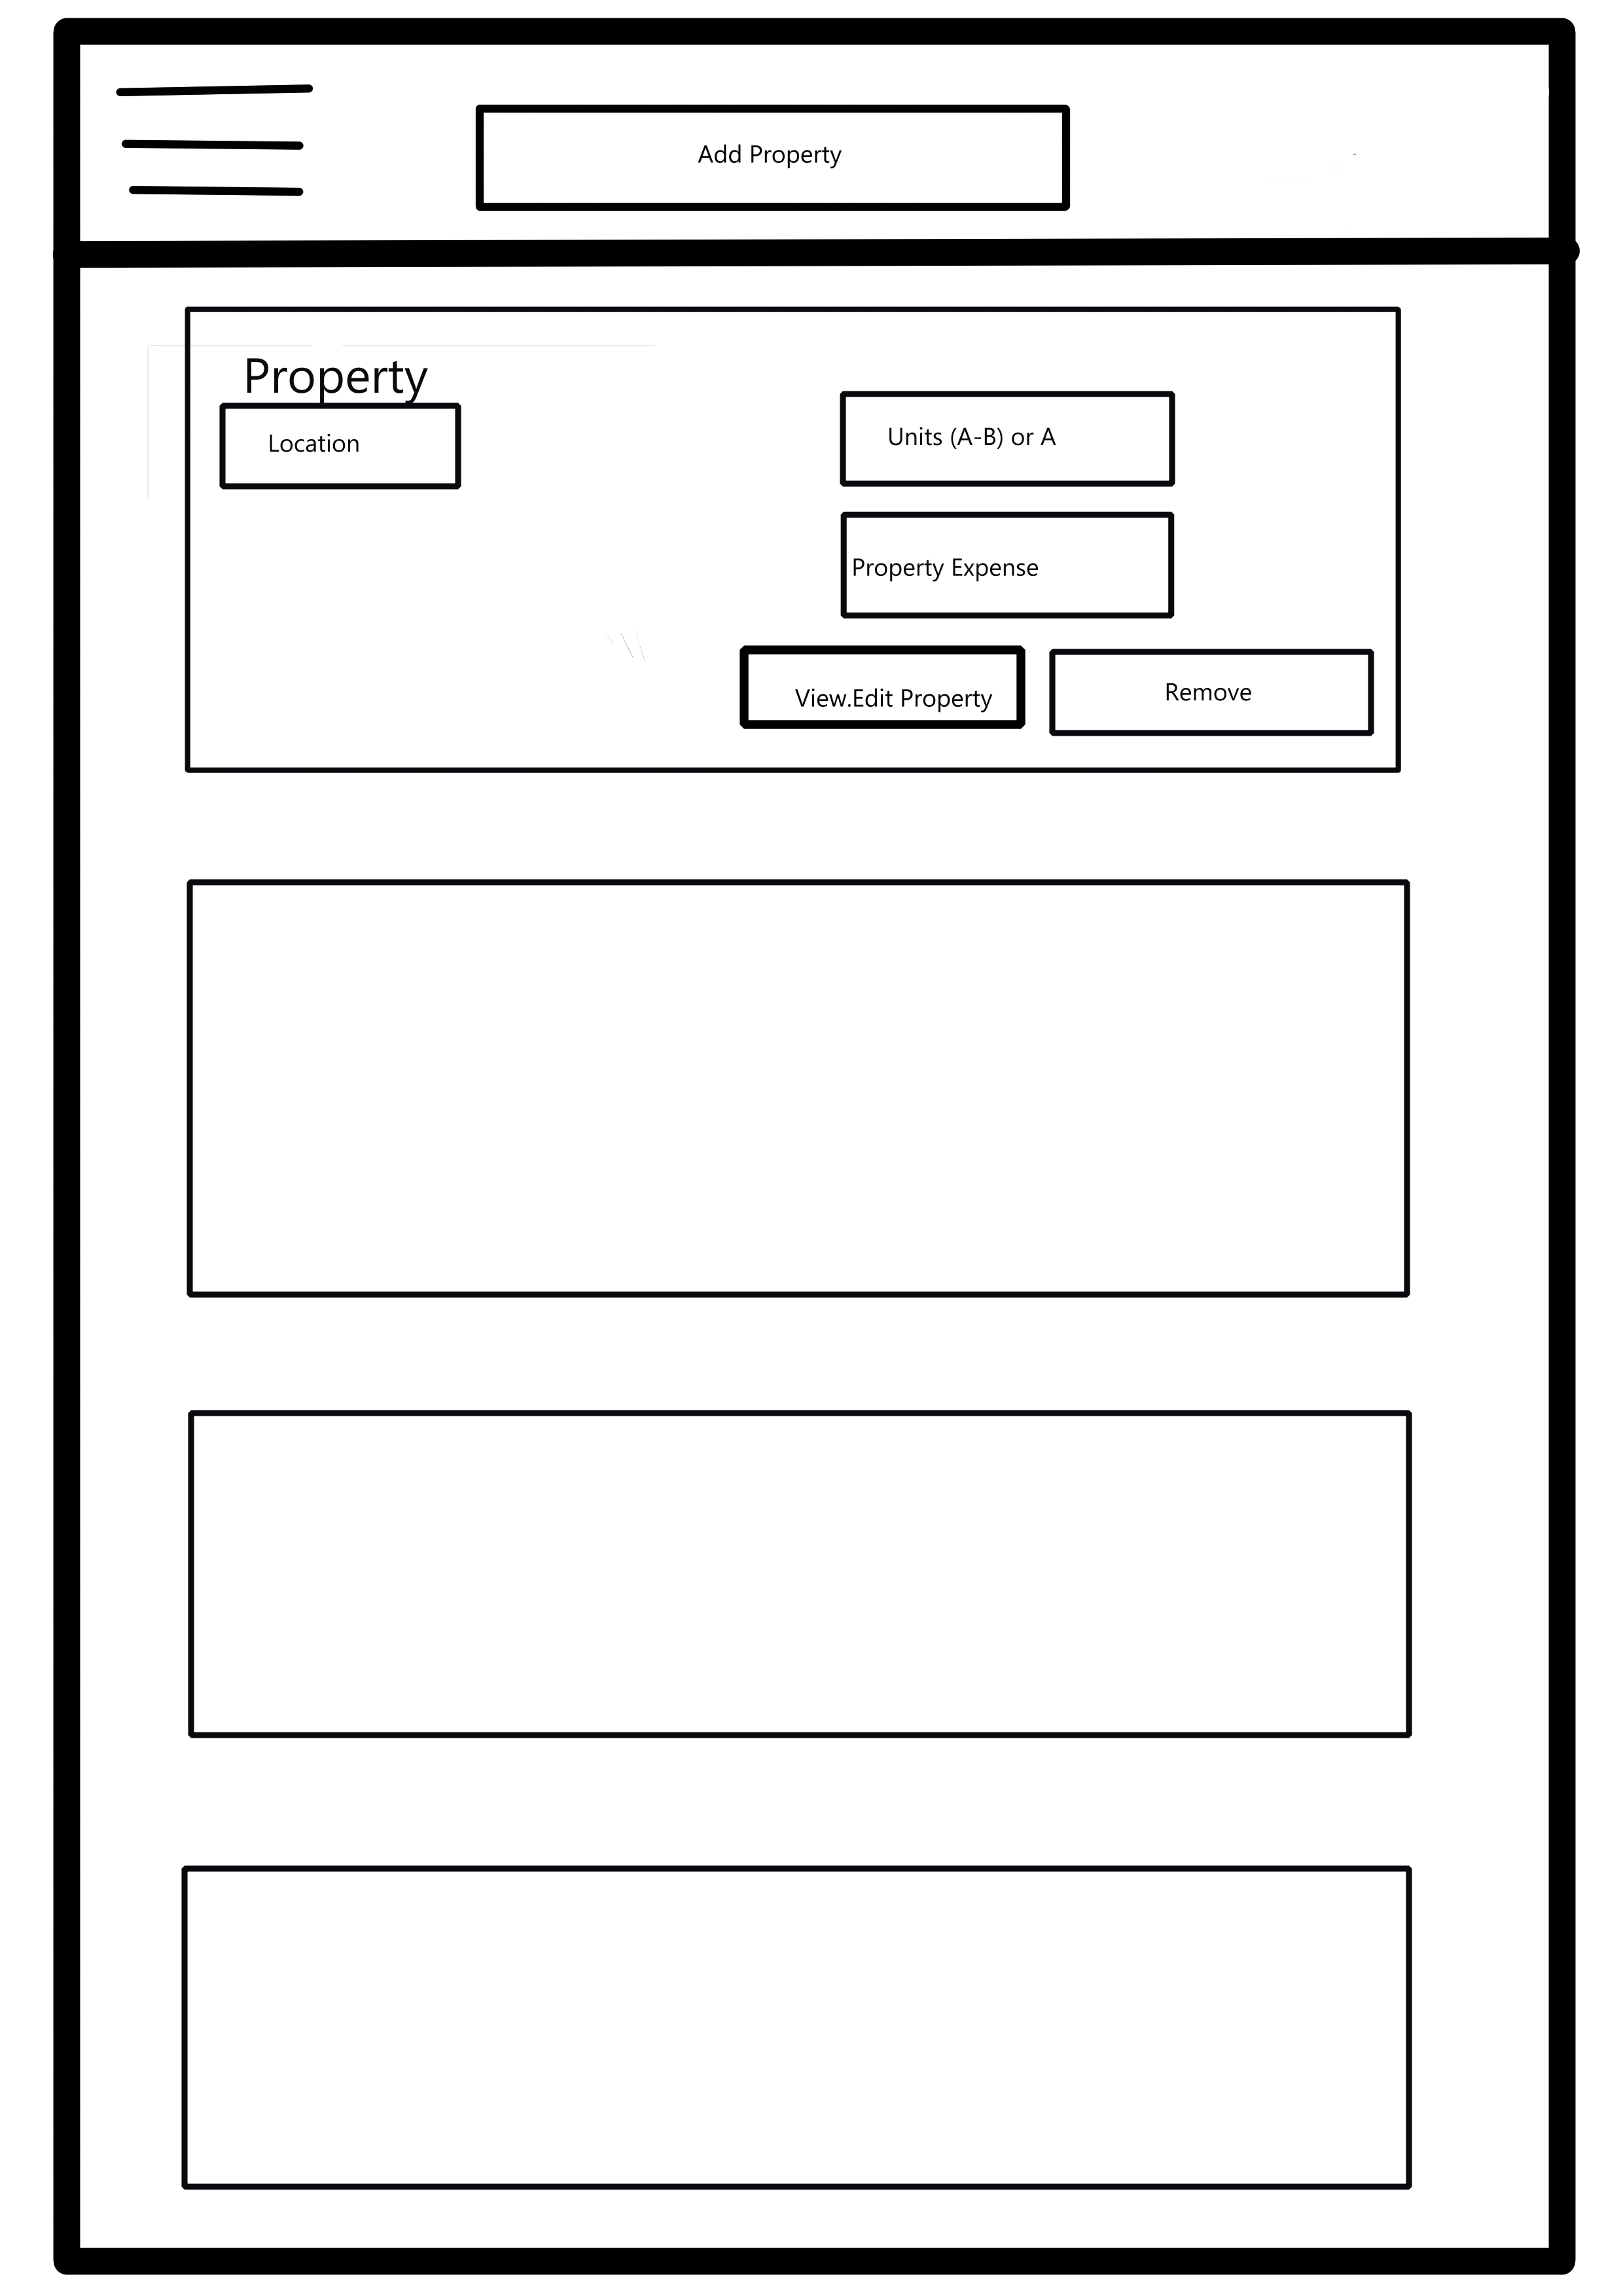
\includegraphics[width=0.5\linewidth]{Property_Managment.png}
                \caption{Property view}
                \label{fig:enter-label}
            \end{figure}
            \begin{figure}
                \centering
                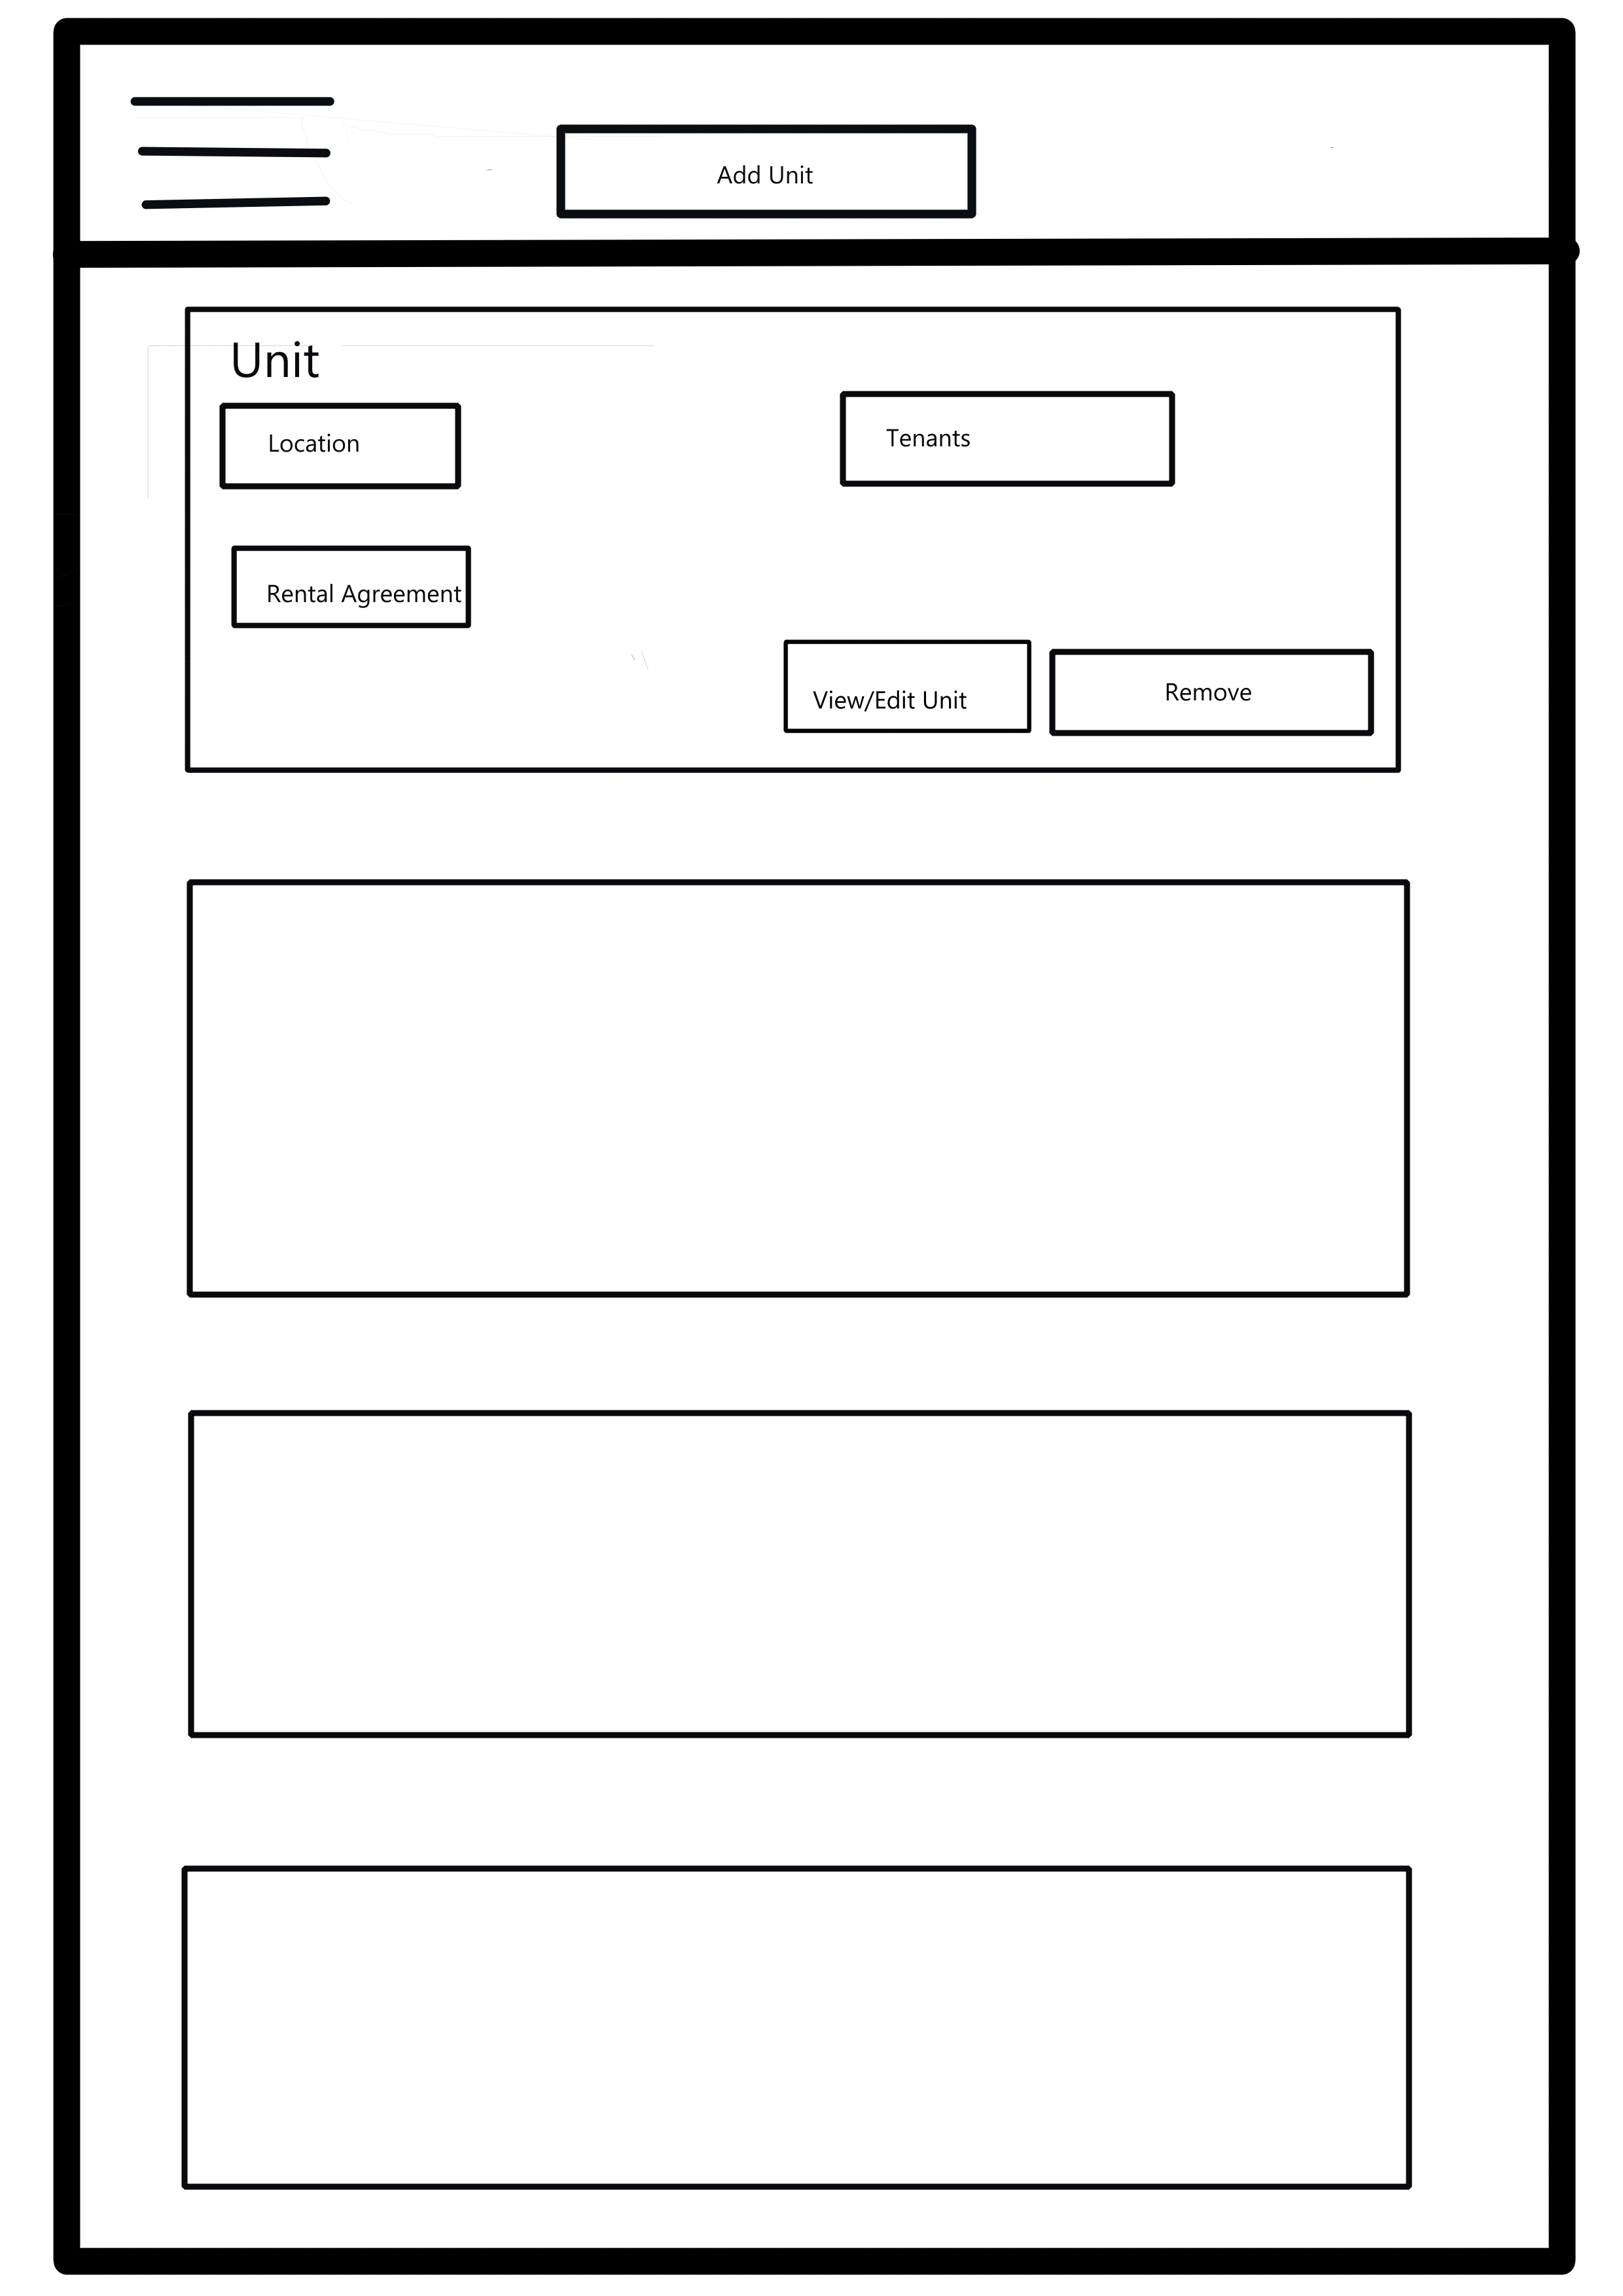
\includegraphics[width=0.5\linewidth]{Unit Managment.png}
                \caption{Unit View}
                \label{fig:enter-label}
            \end{figure}
            \begin{figure}
                \centering
                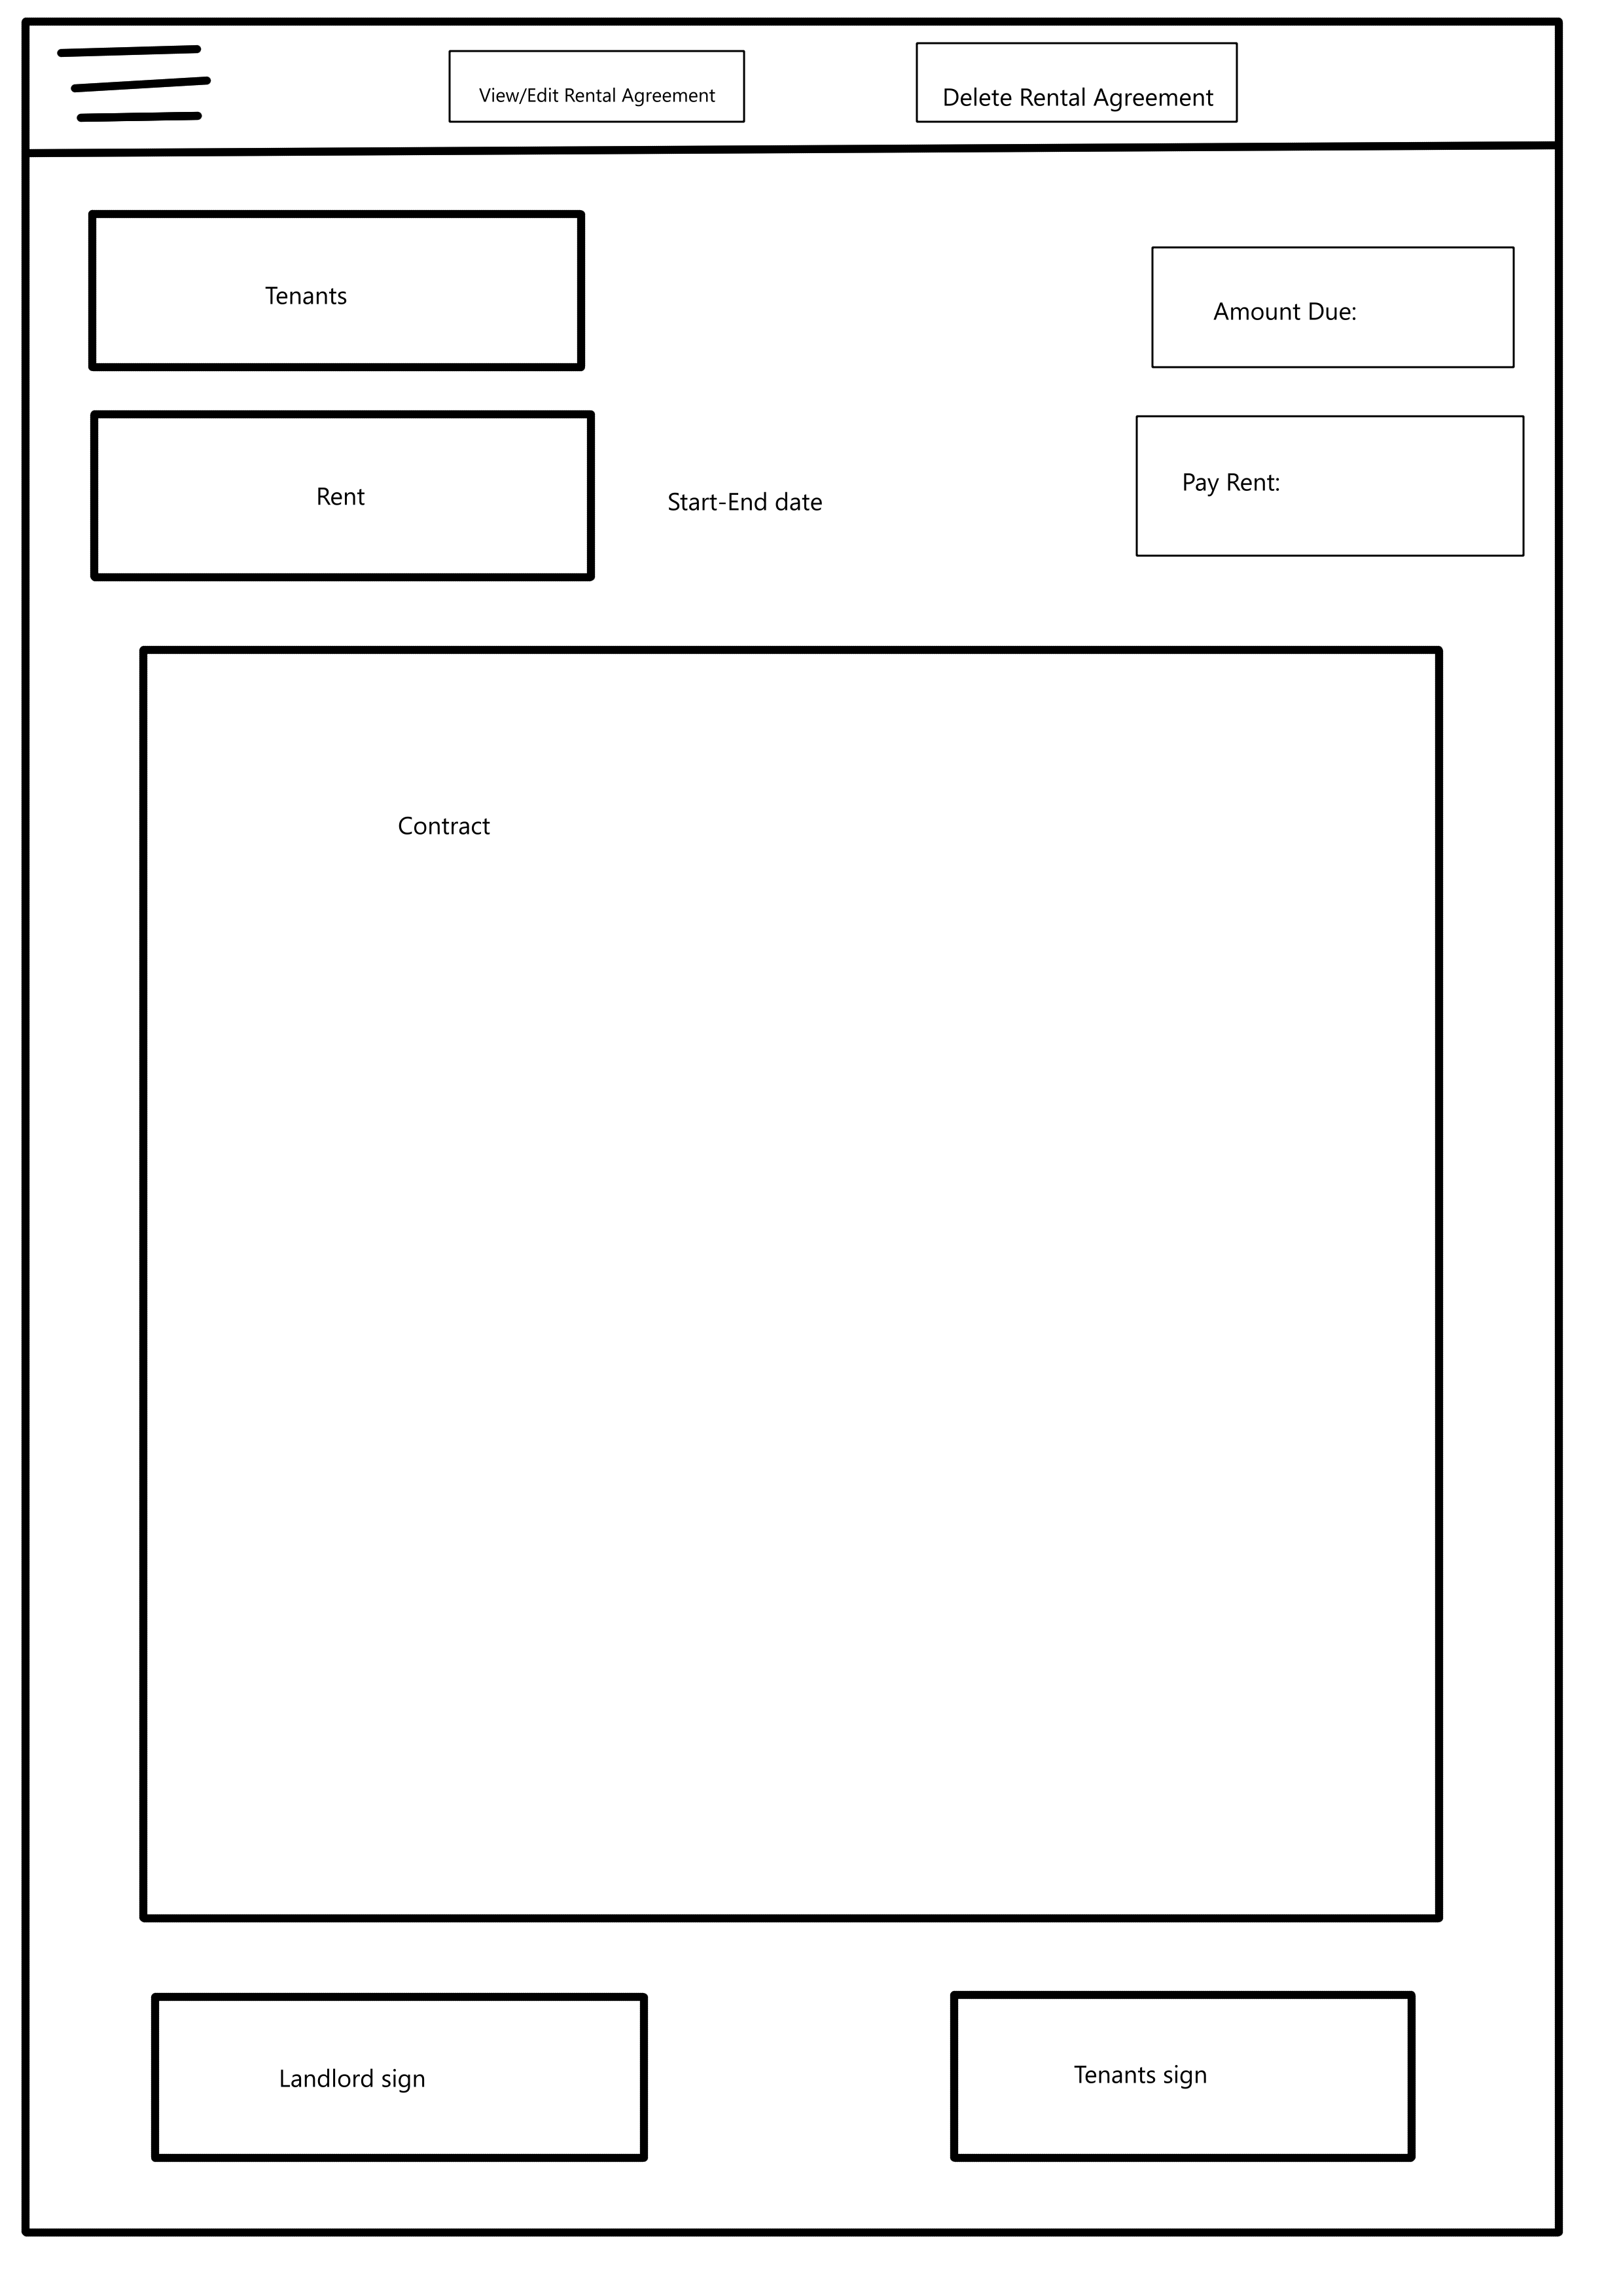
\includegraphics[width=0.5\linewidth]{Rental_Agreement.png}
                \caption{Rental Agreement View}
                \label{fig:enter-label}
            \end{figure}
            
\end{document}

